\documentclass[a4paper,12pt,oneside]{article}
%\documentclass[a4paper,10pt]{scrartcl}

\usepackage[utf8]{inputenc}\usepackage[T2A]{fontenc}
\usepackage[warn]{mathtext}          % русские буквы в формулах, с предупреждением
\usepackage{amsfonts}
\usepackage[english, russian]{babel} % локализация и переносы
\usepackage{indentfirst}   % русский стиль: отступ первого абзаца раздела
\usepackage{misccorr}      % точка в номерах заголовков
\usepackage{cmap}          % русский поиск в pdf
\usepackage{graphicx}      % Работа с графикой \includegraphics{}
\usepackage{psfrag}        % Замена тагов на eps картинкаx
\usepackage{caption2}      % Работа с подписями для фигур, таблиц и пр.
\usepackage{soul}          % Разряженный текст \so{} и подчеркивание \ul{}
\usepackage{soulutf8}      % Поддержка UTF8 в soul
\usepackage{fancyhdr}      % Для работы с колонтитулами
\usepackage{multirow}      % Аналог multicolumn для строк
\usepackage{ltxtable}      % Микс tabularx и longtable
\usepackage{paralist}      % Списки с отступом только в первой строчке
\pretolerance=500         % Отключение переносов слов
\tolerance=500

\usepackage{indentfirst}
\usepackage{misccorr}
\usepackage{graphicx}
\usepackage{amsmath}

\usepackage[perpage]{footmisc} % Нумерация сносок на каждой странице с 1
\usepackage{amsmath}
\usepackage{amsfonts}
\usepackage{pgfplots}
\usepackage{amssymb}
% Задаем отступы: слева 30 мм, справа 10 мм, сверху до колонтитула 10 мм
% снизу 25 мм
% \usepackage[a4paper, top=10mm, left=30mm, right=10mm, bottom=25mm]{geometry}
\usepackage[left=3cm,right=1.5cm,top=2cm,bottom=2cm]{geometry}
% Нумерация формул, картинок и таблиц по секциям
\numberwithin{equation}{section}
\numberwithin{table}{section}
\numberwithin{figure}{section}
% % % % % % % % % % % % % % % % % % % % % % % % % % % % % % % % % % % % % % % % % % % %

\title{Численные методы}
\author{Сергеев Никита Александрович}
\date{15.11.2022 22:50}

\newcommand*\rfrac[2]{{}^{#1}\!/_{#2}}
\newcommand*\absc[1]{|{#1}|}
\DeclareMathOperator\abs{abs}
\begin{document}
\setlength{\abovedisplayskip}{3pt plus 3pt minus 2pt}
\setlength{\abovedisplayshortskip}{3pt plus 2pt minus 3pt}
\setlength{\belowdisplayskip}{3pt plus 3pt minus 2pt}
\setlength{\belowdisplayshortskip}{3pt plus 2pt minus 3pt}
\setlength{\textfloatsep}{1em plus .4em minus .3em}
\setlength{\abovecaptionskip}{0.5em plus .4em minus .1em}
\setlength{\belowcaptionskip}{0.5em plus .4em minus .1em}
\begin{titlepage}
\thispagestyle{empty}
\begin{center}
\LARGE{\textsc{московский государственный университет}} имени \LARGE{\textsc{м.",в.",ломоносова}}\\
\begin{figure}[h]
\centering
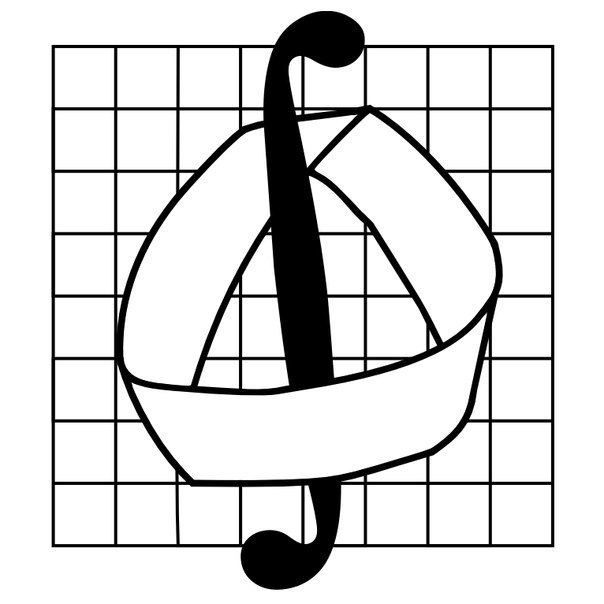
\includegraphics[scale=0.2]{emb.jpg}
\end{figure}
\normalsize Механико-математический факультет\\
\normalsize Кафедра теоретической механики и мехатроники\\
\vspace{4cm}
\Large
Отчёт о проведённой работе по предмету\\
\LARGE{\textbf{«Численные методы и практика на ЭВМ»}}\\[.4em]
\vspace{7cm}
\normalsize
\begin{flushright}
\begin{tabular}{rl}
\textbf{Выполнил:}\\
студент 422 группы\\
кафедры теоретической механики и мехатроники\\
Сергеев Никита Александрович
\end{tabular}
\end{flushright}
\vspace{0.5cm}
\vfill
\vspace{1cm}
{Москва\\
2022}
\end{center}
\end{titlepage}


\begin{titlepage}
\textbf{}
\tableofcontents
\end{titlepage}
\newpage


\section{Постановка задачи}
Рассмотрим задачу оптимального управления: \\
\begin{center}
    $
    \begin{cases}
        \int\limits_0^T (\ddot{x}^2 \cos (\alpha x) - \dot{x}^2 )~dt \to \infty ,\\
        \absc{\ddot{x}} \leq 24 ,\\
        x(0) = 11 ,\\
        \dot{x}(T) = x(T) = 0 ,\\
        \alpha = \{ 0.0; 0.001; 0.01; 0.1\} ,
    \end{cases}
    $
\end{center}
где T - известная константа, параметр задачи. \\

Требуется формализовать задачу как задачу оптимального управления, принципом максимума
Понтрягина свести задачу к краевой задаче, численно решить полученную краевую задачу методом
стрельбы и обосновать точность полученных результатов, проверить полученные экстремали Понтрягина на оптимальность при различных значениях параметра $\alpha = \{ 0.0; 0.001; 0.01; 0.1\}$. \\


\section{Формализация задачи}
Формализуем задачу как задачу оптимального управления. Для этого обозначим $\dot{x} = y$, $\ddot{x} = u$.
Тогда исходная система (1) перепишется в виде: \\
\begin{center}
    $
    \begin{cases}
        \dot{x} = y ,\\
        \dot{y} = u ,\\
        u \in \mathbb{R} ,\\
        x(0) = 11 ,\\
        x(T) = 0 ,\\
        y(T) = 0 ,\\
        \absc{u} \leq 24 ,\\
        \alpha = \{ 0.0; 0.001; 0.01; 0.1\} ,\\
        T = const = 4,\\
        B_0 = \int\limits_0^T (u^2 \cos (\alpha x) - y^2 )~dt \to \infty .\\
    \end{cases}
    $
\end{center}


\section{Система необходимых условий оптимальности}
Выпишем функции Лагранжа и Понтрягина:
\begin{center}

    $\mathcal{L} = \int\limits_0^T L~dt +l$ ,\\
    \begin{tabular}{c c c}
        лагранжиан &$\--$& $L = \lambda_0 (u^2 \cos (\alpha x) - y^2) + p_x(\dot{x}-y) + p_y(\dot{y}-u)$ ,\\
        терминант &$\--$& $l = \lambda_1 (x(0) - 11) + \lambda_2 x(T) + \lambda_3 y(T)$ ,\\
        гамильтониан &$\--$& $H = p_x y + p_y u - \lambda_0 (u^2 \cos (\alpha x) - y^2)$ .\\
    \end{tabular}
\end{center}

Применим к задаче оптимального управления (2) принцип максимума Понтрягина. Необходимые
условия оптимальности:
\begin{enumerate}
    \item уравнения Эйлера-Лагранжа (сопряжённая система уравнений, условие стационарности по $\binom{x}{y}$), 
    $
        \binom{\dot{p}_x}{\dot{p}_y}
        =-
        \left(
            \begin{array}{c}
            \frac{\partial H}{\partial x}
            \vspace{0.15cm} \\
            \frac{\partial H}{\partial y}
            \end{array}
        \right)
    $ : \\
    \begin{center}
        $
        \begin{cases}
            \dot{p}_x = - \alpha \lambda_0 u^2 \sin (\alpha x),\\
            \dot{p}_y = - p_x - 2 \lambda_0 y ;\\
        \end{cases}
        $
    \end{center}
    \item условие оптимальности по управлению, $u = \arg \abs \max\limits_{\absc{u} \leq 24}{H(u)}$: \\
    $u = \arg \abs \max\limits_{\absc{u} \leq 24}{\Big(p_y u - \lambda_0 \big(u^2 \cos (\alpha x)\big)\Big)}$ \\
    
    $ \sqsupset\cos (\alpha x) > 0 \text{: \quad}
    u = \frac{p_y}{2 \lambda_0 \cos (\alpha x)}$, при 
    $
        \lambda_0 \neq 0 
    $, так как парабола $H = -  u^2 \cos (\alpha x) \lambda_0 + p_y u$ с ветвями, направленными вниз ($\lambda_0 \geq 0$), достигает максимума в вершине, при указанном значении аргумента $u$; \\
    $ \sqsupset\cos (\alpha x) < 0 \text{: \quad}
    u = \left[ \begin{array}{c} 24 \\ -24 \end{array} \right.$, при 
    $
        \lambda_0 \neq 0 
    $, так как парабола $H = -  u^2 \cos (\alpha x) \lambda_0 + p_y u$ с ветвями, направленными вверх ($\lambda_0 \geq 0$), достигает максимума в одном из концов; \\
    
    $ \sqsupset\cos (\alpha x) = 0 \text{: \quad}
    u = \forall \beta: \absc{\beta}  \leq 24, \beta \in \mathbb{R} $; \\
    
    \item условия трансверсальности по $\binom{x}{y}$, $p_x(t_k) = (-1)^k\frac{\partial l}{\partial x(t_k)}$, $p_y(t_k) = (-1)^k\frac{\partial l}{\partial y(t_k)}$, где $k = {0; 1}$, $t_0=0$, $t_1=T$: \\
    \begin{center}
     $
        p_y(0) = 0 
    $ \\
    $
        p_x(0) = \lambda_1, p_x(T) = -\lambda_2, p_y(T) = -\lambda_3;
    $
    \end{center}
    
    \item условия стационарности по $t_k$: \\
    нет, так как в задаче $t_k \--$ известные константы; \\
    
    \item условия дополняющей нежёсткости: \\
    нет, так как в задаче отсутствуют условия вида <<меньше или равно>>;
    
    \item условие неотрицательности: $\lambda_0 \geq 0$;
    
    \item условие нормировки (множители Лагранжа могут быть выбраны с точностью до положительного множителя);
    
    \item НЕРОН (множители Лагранжа Не Равны Одновременно Нулю).

\end{enumerate}

\section{Аномальный случай и исследование задачи}
Исследуем возможность аномального случая $\lambda_0 = 0$. При $\lambda_0 = 0$ получим систему дифференциальных уравнений:
    \begin{center}
        $
        \begin{cases}
            \dot{x} = y ,\\
            \dot{y} = u ,\\
            \dot{p}_x = 0,\\
            \dot{p}_y = - p_x;\\
        \end{cases}
        $
    \end{center}
    
Отсюда получаем, $p_x(t) = c, \dot{p}_y(t) = -c$. Так же из условия 2) оптимальности по управлению имеем $p_y \equiv 0$, а значит $\lambda_0 = \lambda_1 = \lambda_2 = \lambda_3 = 0$, что противоречит условию 8) НЕРОН.\\

В силу условия 7) можно выбрать $\lambda_0=\rfrac{1}{2}$, тогда обозначим $\cos (\alpha x) = g(\alpha, x)$ и управление преобразуется в $u=$
$\left[ 
\begin{tabular}{c c} 
$\rfrac{p_y}{g(\alpha, x)}$ & $g(\alpha, x) > 0$, \\
$\left[ \begin{array}{c} 24 \\ -24 \end{array} \right.$ & $g(\alpha, x) < 0$, \\
$\forall \beta: \absc{\beta}  \leq 24, \beta \in \mathbb{R}$ & $g(\alpha, x) = 0$;
\end{tabular} 
\right.$

\section{Краевая задача}
    Таким образом, на основе принципа максимума Понтрягина задача оптимального управления сводится к краевой задаче. Итого имеем:
\begin{center}
    $
    \begin{cases}
        \dot{x} = y ,\\
        \dot{y} = u ,\\
        \dot{p}_x = - \frac{\alpha}{2} u^2 \sin (\alpha x),\\
        \dot{p}_y = - p_x - y ;\\
    \end{cases}
    $ \\
    \begin{tabular}{c c}
        $x(0) = 11$, & $x(T) = 0$,\\
        $p_y(0) = 0$, & $y(T) = 0$,\\
        $T \equiv 4$, & $\alpha = \{ 0.0; 0.001; 0.01; 0.1\}$.\\
    \end{tabular}\\
\end{center}

\section{Численное решение методом стрельбы}
Краевая задача решается численно методом стрельбы. В качестве параметров пристрелки выбираются недостающие для решения задачи Коши значения при $t=0$: $\alpha_1 = y(0),\text{ } \alpha_2 = p_x(0)$. Задав эти значения каким-либо образом и решив задачу Коши на отрезке  $\left[0;\text{ }T\right]$, получим соответствующие выбранному значению $\vec{\alpha}:=\{\alpha_1;\text{ }\alpha_2\}$ функции $x(\cdot)[\vec{\alpha}],\text{ }y(\cdot)[\vec{\alpha}],\text{ }p_x(\cdot)[\vec{\alpha}],\text{ }p_y(\cdot)[\vec{\alpha}],\text{ }$и, в частности, значения $x(T)[\vec{\alpha}],\text{ }y(T)[\vec{\alpha}]$. Задача Коши для системы дифференциальных
уравнений, начальных условий в 0 момент времени и условий $y(0) = \alpha_1$, $p_x (0) = \alpha_2$ решается
численно явным методом Рунге-Кутты 8-го порядка, основанным на расчётных формулах Фельберга с автоматическим выбором шага (то есть с контролем относительной локальной погрешности на шаге по правилу Рунге). Для решения краевой задачи необходимо подобрать значения $\alpha_1$, $\alpha_2$ так, чтобы выполнились условия:
$
\begin{array}{c}
    x(T)[\vec{\alpha}]=0,\\
    y(T)[\vec{\alpha}]=0.\\
\end{array}
$\\
Cоответственно вектор-функцией невязок будет функция $
X(\vec{\alpha})=
\left(
    \begin{array}{c}
        x(T)[\vec{\alpha}]\\
        y(T)[\vec{\alpha}]
    \end{array}
\right)
$. Таким образом, в результате выбора вычислительной схемы метода стрельбы, решение краевой задачи свелось к реше-
нию системы двух алгебраических уравнений от двух неизвестных. Корень $\vec{\alpha}$ системы алгебраических
уравнений $X(\vec{\alpha})=0$ находится методом Ньютона с модификацией Исаева-Сонина. Решение линейной системы уравнений внутри модифицированного метода Ньютона осуществляется методом Гаусса с выбором главного элемента по столбцу, с повторным пересчётом.\\

Схема численного решения краевой задачи методом стрельбы выбрана таким образом, что при отсутствии ошибок в программной реализации решения задачи Коши, найденный методом Ньютона корень будет правильным (без учёта погрешности численного интегрирования), даже если внутри метода Ньютона есть какие-то ишибки. Напротив, ошибка в решении задачи Коши делает бесполезным полученный результат, даже если всё остальное запрограммировано правильно и методу Ньютона
удалось найти корень.\\

Исходя из этого крайне важен следующий тест части программы, решающей задачу Коши, на
системе дифференциальных уравнений с известным аналитическим решением.

\section{Тест решения задачи Коши:\\ гармонический осциллятор}
\end{document}
